% !TEX root = ../thesis.tex
% !TEX spellcheck = en-US

\thispagestyle{empty}

\section{Experimental Results}
\label{sec:Experimental Results}

With the final problem definition and dataset in place a series of experiments were conducted to evaluate the performance of the different approaches explained in Section~\ref{sec:Methods}.
This part of the thesis lays out these experiments and their results. First the research objectives will be reiterated. Next the experimental setup for each of the methods will be described and the outcomes and observations will be presented.

\subsection{Objectives}
\label{sub:Objectives}

The experiments had simple objectives: The goal was to evaluate each method in terms of its effectiveness using a prediction metric well-suited for this problem. The metric used was \gls{MCC} as described in Section~\ref{sub:Performance Metric: Matthews Correlation Coefficient}. Effectiveness in particular meant comparing the algorithms with regards to their overall performance on test data and their ability to generalize well, i.e. to be robust against overfitting.
% Further considerations were taken into account such as the simplicity of the model in terms of model assumptions but also ease of use and interpretability, as well as algorithmic time and space complexity requirements.


\subsection{Baseline}
\label{sub:Baseline}

In order to have a reference point for predictive performance that any method should surpass two guessing strategies were used, namely uniform and stratified guessing. Uniform guessing means sampling from a uniform distribution, commonly known as ``rolling dice'', while stratified guessing refers to an estimator that samples a label for a data point using the observed distribution of labels in the data. Both methods effectively ignore the data itself when producing labels and as such any predictive algorithm should do better.

Averaged over 1000 runs both strategies yielded an \gls{MCC} score close to zero. Accuracy by comparison was around 0.16 for uniform guessing and 0.26 for stratified guessing. These results are within our expectations and further highlight the rationale for choosing \gls{MCC} as the principal metric: \gls{MCC} is zero for uninformed predictions for either strategy whereas the accuracy in the uniform setting corresponds simply to a value of $1/k$ where $k = 6$ is the number of labels. The accuracy in the stratified setting reveals improves by taking advantage of knowledge about the skew in the label distribution. Figure~\ref{fig:guessing-conf-matrix} shows the confusion matrices for these baseline variants in absolute and normalized form, where the described properties these guessing strategies can be observed.

\begin{figure}
 % From http://localhost:8888/notebooks/thesis/experiments/vector-space-models/Vector%20Space%20Models.ipynb#Baseline:-Guessing-Strategies
    \centering
    \begin{subfigure}[b]{0.47\textwidth}
        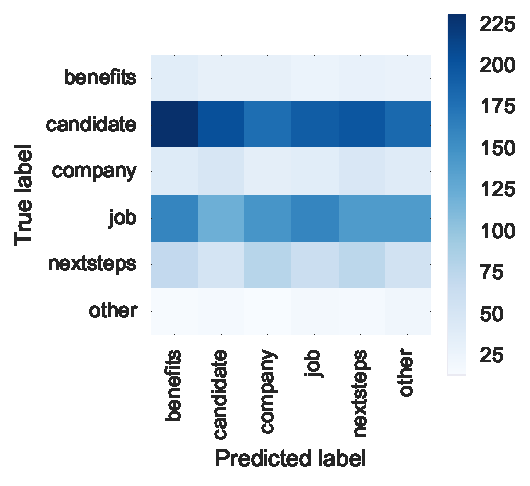
\includegraphics[width=\textwidth]{img/exp-vector-space/guessing-conf-matrix-uniform.pdf}
        \caption{Uniform guessing}
\label{fig:guessing-conf-matrix-uniform}
    \end{subfigure}
~\begin{subfigure}[b]{0.48\textwidth}
        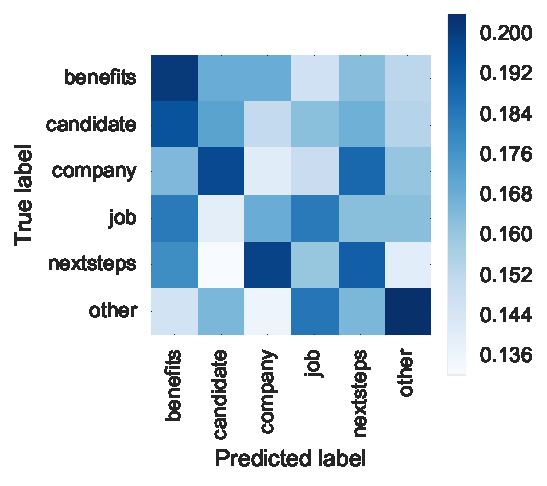
\includegraphics[width=\textwidth]{img/exp-vector-space/guessing-conf-matrix-uniform-normalized.pdf}
        \caption{Uniform guessing (normalized)}
\label{fig:guessing-conf-matrix-uniform-normalized}
    \end{subfigure}
~\begin{subfigure}[b]{0.47\textwidth}
        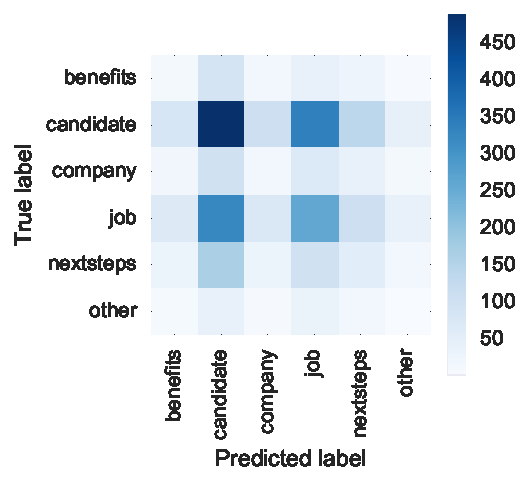
\includegraphics[width=\textwidth]{img/exp-vector-space/guessing-conf-matrix-stratified.pdf}
        \caption{Stratified guessing}
\label{fig:guessing-conf-matrix-stratified}
    \end{subfigure}
~\begin{subfigure}[b]{0.48\textwidth}
        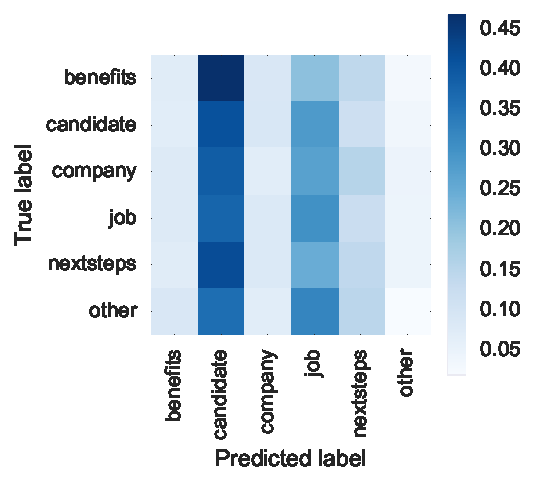
\includegraphics[width=\textwidth]{img/exp-vector-space/guessing-conf-matrix-stratified-normalized.pdf}
        \caption{Stratified guessing (normalized)}
\label{fig:guessing-stratified-normalized}
    \end{subfigure}
    \caption{Confusion matrices of uniform and stratified guessing strategies.}
\label{fig:guessing-conf-matrix}
\end{figure}

\clearpage

\subsection{Classification With Vector Space Models}
\label{sub:Classification With Vector Space Models}

A popular way to approach text classification and other tasks in natural language processing is to build a model that maps data into a vector space. Distance between data points in this space then translates to similarity between the objects (see Section~\ref{sub:Vector Space Models}).
The resulting vector representation of the data can then be fed into various learning algorithms. This section describes the experiments performed to evaluate such approaches.

First the different methods to produce such vector spaces are compared. Several methods were used to generate vectors from the data while limiting dimensionality to 300 for comparability --- a heuristically chosen value as performance for the models did not increase significantly beyond it. These vector representations were then compared in terms of performance by using them as input to the simple classification model Logistic Regression.
Second, the best performing configurations for each type of method were chosen and a set of various classification techniques were applied to them which were described previously in Section~\ref{sub:Methods For Classification With Vector Space Models}.

\subsubsection{N-gram Models}
\label{subs:N-gram Models (Experimental Results)}

The first class of language models that was investigated for the task of multi-class classification are N-gram models that were explained in Section~\ref{subs:N-gram Models (Methods)}.
N-gram models come in a variety of forms. In these experiments the most common variants were set up as hyper-parameters to the model as  listed in Table~\ref{tab:N-gram Hyper-parameters Space}.

\begin{table}[h]
  \begin{center}
  \begin{tabular}{ l l l}
    \toprule
    Hyper-Parameter & N-gram Type: Words & N-gram Type: Characters \\
    \midrule
    N-gram Range (Range) & [1,1], [1,2], [1,3], [2,3], [3,3] & [1,5], [1,10], [5,10], [5,15] \\
    Stop Words & English, None & --- \\
    Vector Size (Size) & 10, 100, 300 & 10, 100, 300 \\
    IDF & Yes, No & Yes, No \\
    Norm & L1, L2, None & L1, L2, None \\
    Sub-linear TF & Yes, No & Yes, No \\
    \bottomrule
  \end{tabular}
  \caption{Parameter search space for word and character level N-gram models}
\label{tab:N-gram Hyper-parameters Space}
\end{center}
\end{table}

A grid search was performed to test all combinations of configurations within this hyper-parameter space. Each configuration was evaluated with regards to its \gls{MCC} score using 5-fold cross-validation on the training data with three standard classifiers: Logistic Regression and Naive Bayes and SVM.
Table~\ref{tab:Ngram Grid Search} shows the five best results of the exhaustive grid search over the hyper-parameter configurations.

\begin{table}[h]
  \begin{center}
  \begin{tabular}{ l l l l l l l l }
    \toprule
    Type & Range & Stop words & Size & IDF & Norm & Sub-linear TF & \gls{MCC} \\
    \midrule
    Word & [1,1] & None & 300 & Yes &  & Yes & 0.689 \\
    Word & [1,1] & None & 300 & Yes &  & No & 0.687 \\
    Word & [1,1] & None & 300 & No &  & Yes & 0.682 \\
    Word & [1,1] & None & 300 & No &  & No & 0.682 \\
    Word & [1,1] & None & 300 & Yes & L2 & Yes & 0.68 \\
    \midrule
    Word & [1,1] & None & 300 & No & & Yes & 0.659  \\
    Word & [1,1] & None & 300 & No & & No & 0.656 \\
    Word & [1,2] & None & 300 & No & & Yes & 0.655 \\
    Word & [1,2] & None & 300 & No & & No & 0.655 \\
    Word & [1,3] & None & 300 & No & & No & 0.65 \\
    \midrule
    Word & [1,1] & None & 300 & Yes & & Yes & 0.689 \\
    Word & [1,1] & None & 300 & Yes & & No  & 0.689 \\
    Word & [1,2] & None & 300 & Yes & & Yes & 0.677 \\
    Word & [1,2] & None & 300 & Yes & & No  & 0.677 \\
    Word & [1,3] & None & 300 & Yes & & Yes & 0.674 \\
    \bottomrule
  \end{tabular}
  \caption{Top 5 results of grid search over hyper-parameter space using 5-fold cross-validation on the training set with Logistic Regression (top), Naive Bayes (middle) and SVM (bottom).}
\label{tab:Ngram Grid Search}
\end{center}
\end{table}

The effects of the different hyper-parameters on performance can be observed based on these results. Regarding the N-gram \emph{type}, words as the atomic unit for N-grams consistently led to better results. This is due to the fact that the search space of combinations of characters is significantly larger than the search space of known words, so model complexity increases exponentially.
With regards to the \emph{range}, i.e.\ the interval for possible $N$ in N-grams, there are slight differences to be observed between the three classifiers used, but with all three models the best performance is achieved using Unigrams. Also all of the top results across all classifiers include Unigrams in the model while some extend the range towards bigrams or trigrams.
None of the top results of the performed grid searches used \emph{stop words}. This is interesting as using stop-words to remove hand-picked, highly frequent words that do not carry much meaning is common practice.
When it comes to the \emph{size} of vectors, for the given settings the highest vector dimensionality of 300 achieves the best performance.
There is no consensus between the classifiers on whether or not to weigh the N-gram frequencies by the inverse document frequency (\emph{IDF}, see Section~\ref{subp:TF.IDF weighting}). With respect to the \emph{norm} used, in these experiments normalizing vectors decreased performance. Only in the fifth best performing configuration when using Logistic Regression vectors were normalized, in this case using the L2 norm.
Lastly applying sub-linear term frequency scaling (\emph{Sub-linear TF}, see Section~\ref{subp:Sublinear TF scaling}) did not seem to affect the results significantly and about half of the top results were obtained using this technique.

Based on these observations the best model for each classifier with regards to \gls{MCC} validation score was chosen and trained on the whole training data and tested on the test data set to estimate the final performance. Table~\ref{tab:Ngram Grid Search Scores} shows the scores of each classifier using these best N-gram models. It is evident that here logistic regression performs best, achieving the highest \gls{MCC} score as well as good accuracy.

\begin{table}
  \begin{center}
  \begin{tabular}{ r | *2l | *2l }
    \toprule
     & \multicolumn{2}{c|}{Training} & \multicolumn{2}{c}{Test}\\
    Classifier & Accuracy & MCC & Accuracy & MCC \\
    \midrule
    Logistic Regression & 0.824 & 0.761 & 0.787 & 0.708 \\
    Naive Bayes         & 0.769 & 0.681 & 0.767 & 0.677 \\
    SVM                 & 0.835 & 0.681 & 0.786 & 0.700 \\
    \bottomrule
  \end{tabular}
  \caption{Performance of each best N-gram model with Logistic Regression and Naive Bayes on the test data.}
\label{tab:Ngram Grid Search Scores}
\end{center}
\end{table}

\begin{figure}
    \centering
    \begin{subfigure}[b]{0.3595\textwidth}
        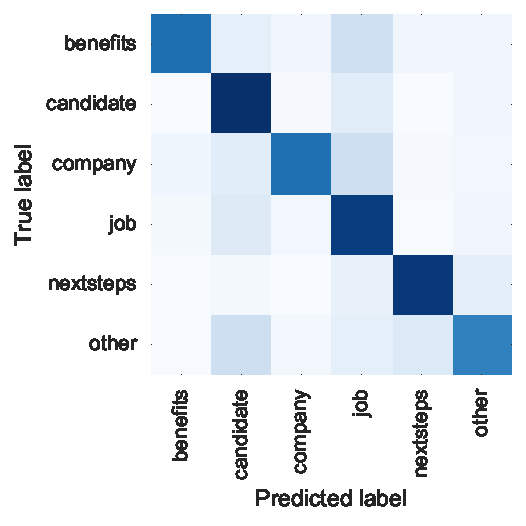
\includegraphics[width=\textwidth]{img/exp-vector-space/ngram-conf-matrix-logreg-normalized.pdf}
        \caption{Logistic Regression}
\label{fig:ngram-conf-matrix-logreg-normalized}
    \end{subfigure}
    \begin{subfigure}[b]{0.267\textwidth}
        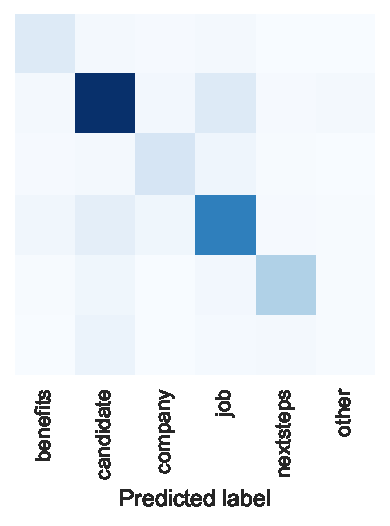
\includegraphics[width=\textwidth]{img/exp-vector-space/ngram-conf-matrix-naivebayes-normalized.pdf}
        \caption{Naive Bayes}
\label{fig:ngram-conf-matrix-naivebayes-normalized}
    \end{subfigure}
    \begin{subfigure}[b]{0.35\textwidth}
        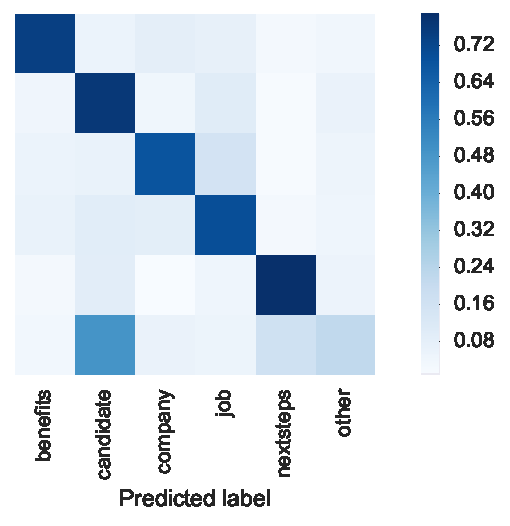
\includegraphics[width=\textwidth]{img/exp-vector-space/ngram-conf-matrix-svm-normalized.pdf}
        \caption{SVM}
\label{fig:ngram-conf-matrix-svm-normalized}
    \end{subfigure}
    \caption{Normalized confusion matrices all three classifiers using the best N-gram model found via cross-validated grid search. Both Naive Bayes as well as SVM show label bias towards the prevalent class \emph{candidate}.}
\label{fig:ngram-conf-matrix}
\end{figure}

To understand the mapping of the data in the resulting vector space visualizations were produced using \gls{PCA} and \gls{t-SNE}. The results for best-performing N-gram model can be seen in Figure~\ref{fig:ngram pca and tsne}. Especially the \gls{PCA} visualization shows that a high percentage of the data for each class can be separated from other classes even with a linear model.

\begin{figure}[h]
    \centering
    \begin{subfigure}[b]{0.48\textwidth}
      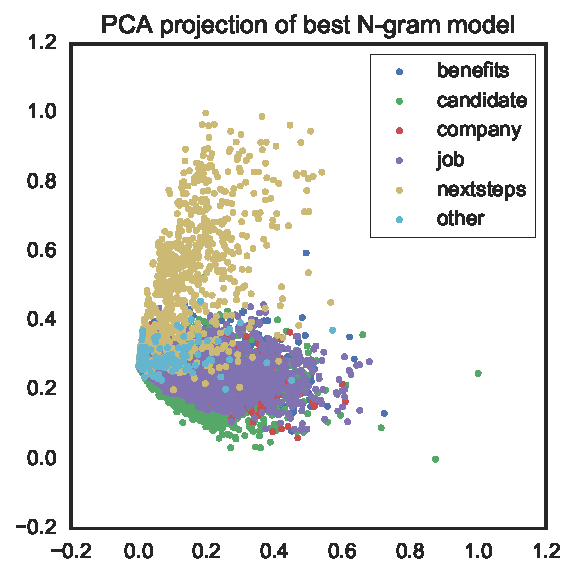
\includegraphics[width=\textwidth]{img/exp-vector-space/ngram-pca.pdf}
      \caption{PCA projection}
\label{fig:ngram-pca}
    \end{subfigure}
~
    %add desired spacing between images, e. g. ~, \quad, \qquad, \hfill etc.
    %(or a blank line to force the subfigure onto a new line)
    \begin{subfigure}[b]{0.48\textwidth}
      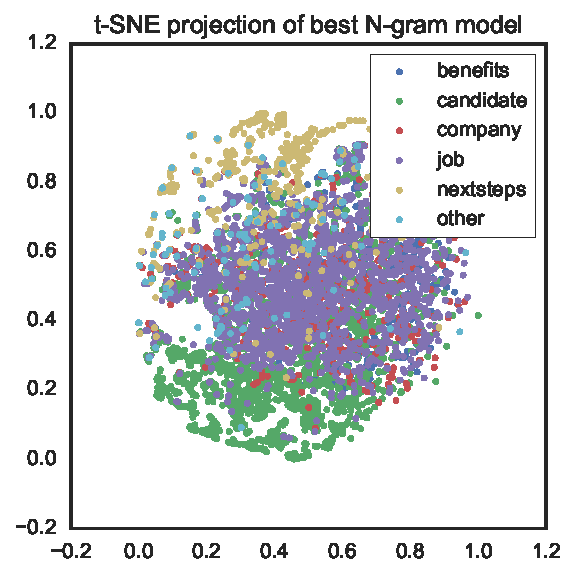
\includegraphics[width=\textwidth]{img/exp-vector-space/ngram-tsne.pdf}
      \caption{t-SNE projection}
\label{fig:ngram-tsne}
    \end{subfigure}
    \caption{Document vectors produced by the best N-gram model (optimized w.r.t. Logistic Regression) projected onto the first 2 principal components (left) and project using t-SNE projection.}
\label{fig:ngram pca and tsne}
\end{figure}

\subsubsection{Bag-of-Means: An Averaged Word2Vec Model}
\label{subs:Bag-of-Means: An Averaged Word2Vec Model}

Next a Bag-of-Means model as described in Section~\ref{subp:Bag-of-Means} was evaluated with the same set of classifiers. The model was evaluated on the same test and training data split as used for the N-gram model above. The results are shown in Table~\ref{tab:Bag-Of-Means Results}.

\begin{table}[h]
  \begin{center}
  \begin{tabular}{ r | *2l | *2l }
    \toprule
     & \multicolumn{2}{c|}{Training} & \multicolumn{2}{c}{Test}\\
    Classifier & Accuracy & MCC & Accuracy & MCC \\
    \midrule
    Logistic Regression & 0.797 & 0.722 & 0.784 & 0.702 \\
    Naive Bayes         & 0.337 & 0.271 & 0.320 & 0.251 \\
    SVM                 & 0.545 & 0.356 & 0.562 & 0.379 \\
    \bottomrule
  \end{tabular}
  \caption{Performance base classifiers using the Bag-of-Means model}
\label{tab:Bag-Of-Means Results}
\end{center}
\end{table}

As a basis, pre-trained word vectors from the Google News dataset\footnote{The dataset contains contains 300-dimensional vectors for 3 million words and phrases. The phrases were obtained using a simple data-driven approach described in~\cite{Mikolov:2013ab}. The dataset can be obtained on the following website: \url{https://code.google.com/archive/p/word2vec/}} were extracted for the words that occur in the dataset.
Then for each sentence in the data a sentence vector was obtained by taking the arithmetic mean over the vectors for all words in the sentence. Labels were again predicted using Logistic Regression, Naive Bayes and SVM.
We can see that the model performs well using Logistic Regression and it is almost on par with the best N-gram model. On the other hand the variance in results between the classifiers is drastic, and Naive Bayes' score is 0.451 lower that Logistic Regression in absolute terms. The confusion matrices in Figure~\ref{fig:bom-conf-matrix} reveal strong label bias in the case of Naive Bayes and SVM.

\begin{figure}[h]
    \centering
    \begin{subfigure}[b]{0.365\textwidth}
        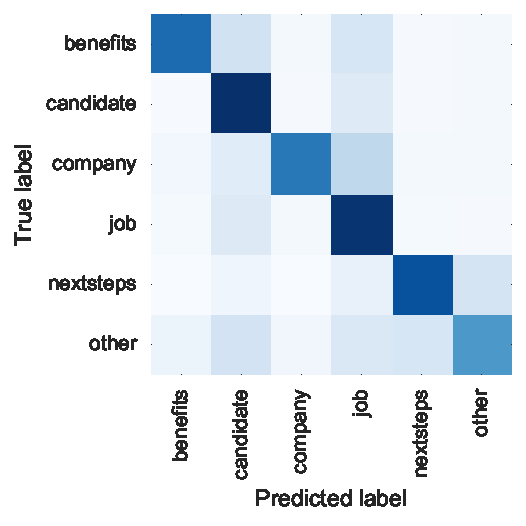
\includegraphics[width=\textwidth]{img/exp-vector-space/bom-conf-matrix-logreg-normalized.pdf}
        \caption{Logistic Regression}
\label{fig:bom-conf-matrix-logreg-normalized}
    \end{subfigure}
    \begin{subfigure}[b]{0.27\textwidth}
        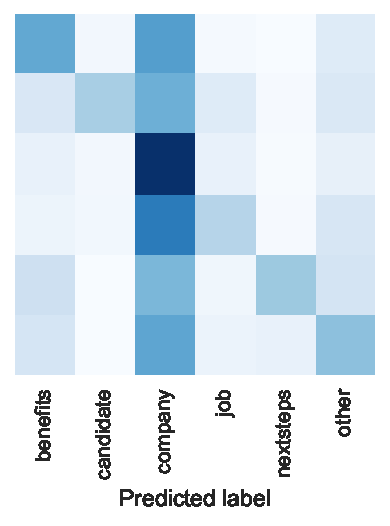
\includegraphics[width=\textwidth]{img/exp-vector-space/bom-conf-matrix-naivebayes-normalized.pdf}
        \caption{Naive Bayes}
\label{fig:bom-conf-matrix-naivebayes-normalized}
    \end{subfigure}
    \begin{subfigure}[b]{0.345\textwidth}
        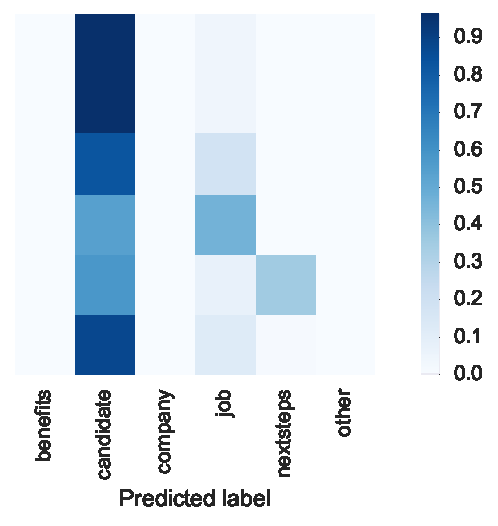
\includegraphics[width=\textwidth]{img/exp-vector-space/bom-conf-matrix-svm-normalized.pdf}
        \caption{SVM}
\label{fig:bom-conf-matrix-svm-normalized}
    \end{subfigure}
    \caption{Normalized confusion matrices of all three classifiers using the Bag-of-Means model.}
\label{fig:bom-conf-matrix}
\end{figure}

The visualization in Figure~\ref{fig:bom} shows a projection of the vectors into a 2 dimensional space. We can visually confirm that labels tend to cluster in this space.

\begin{figure}[h!]
    \centering
    \begin{subfigure}[b]{0.48\textwidth}
      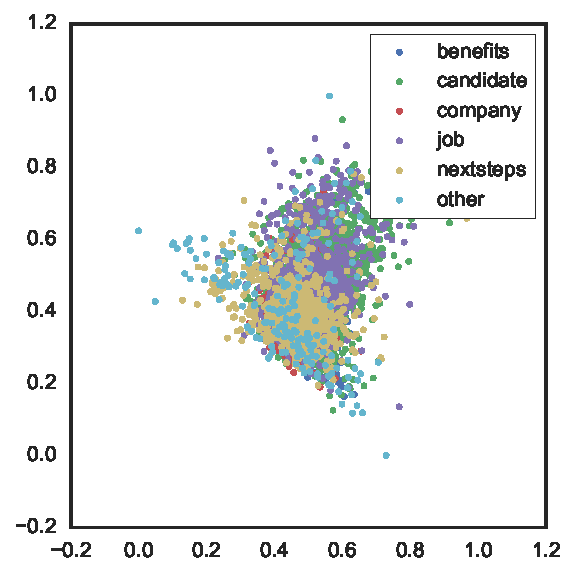
\includegraphics[width=\textwidth]{img/exp-vector-space/bom-pca.pdf}
      \caption{PCA projection}
\label{fig:bom-pca}
    \end{subfigure}
~
    %add desired spacing between images, e. g. ~, \quad, \qquad, \hfill etc.
    %(or a blank line to force the subfigure onto a new line)
    \begin{subfigure}[b]{0.48\textwidth}
      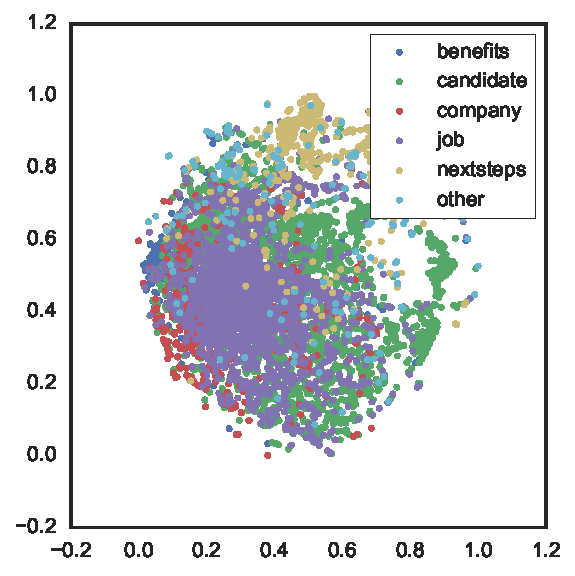
\includegraphics[width=\textwidth]{img/exp-vector-space/bom-tsne.pdf}
      \caption{t-SNE projection}
\label{fig:bom-tsne}
    \end{subfigure}
    \caption{Document vectors produced by Bag-of-Means model (optimized w.r.t. Logistic Regression) projected onto the first 2 principal components (left) and projected using t-SNE projection. }
\label{fig:bom}
\end{figure}

\subsubsection{Paragraph Vectors using Distributed Representations}
\label{subs:Paragraph Vectors using Distributed Representations}

\todo{Doc2Vec model is evaluated in 2 ways (normal and trained on inferred vectors)}

Next a vector space model was build using the approach proposed by~\cite{Le:2014aa} and described in detail in Section~\ref{subp:Paragraph Vectors}. There are several variants and hyper-parameters to this model and their effect was experimentally evaluated. As this model is computationally quite expensive a grid search as for the N-gram model above was infeasible. Hence performance effects were measured by varying the hyper-parameters one at a time while keeping the others fixed. In this process Logistic Regression was used with 5-fold cross-validation. All Paragraph Vector models were tested with both the trained vectors as well as vectors inferred at prediction time. The default configuration can be seen in Table ~\ref{tab:Paragraph Vector Defaults} below.

\begin{table}[h]
  \begin{center}
  \begin{tabular}{ l | l }
    \toprule
    Vector Size & 100 \\
    Sub-sampling threshold & No \\
    Hierarchical Softmax & Yes \\
    Negative Sampling Value & 3 \\
    Window Size & 10 \\
    Model Type & PV-DBOW \\
    Training Type & Inferred Vectors \\
    \bottomrule
  \end{tabular}
  \caption{Default hyper-parameter configuration for Paragraph Vectors}
  \label{tab:Paragraph Vector Defaults}
\end{center}
\end{table}

\begin{table}[h]
  \begin{center}
    \begin{tabular}{ c | c | c | c }
      \toprule
      Hyper-Parameter & Setting & Training Score & Test Score \\
      \midrule
      \multirow{4}{*}{Vector Size}
       & 2 & 0.229 & 0.223 \\
       & 10  & 0.545 & 0.541 \\
       & 100 & 0.614 & 0.589 \\
       & 300 & 0.648 & \textbf{0.608} \\
      \midrule
      \multirow{4}{*}{Sub-sampling Threshold}
       & None & 0.611 & \textbf{0.588} \\
       & 1e-4 & 0.495 & 0.475 \\
       & 1e-5 & 0.328 & 0.303 \\
       & 1e-6 & 0.149 & 0.127 \\
      \midrule
      \multirow{2}{*}{Hierarchical Softmax}
       & Not used & 0.600 & 0.578 \\
       & Used     & 0.613 & \textbf{0.586} \\
      \midrule
      \multirow{4}{*}{Negative Sampling Value}
       & 0 & 0.598 & 0.575 \\
       & 2 & 0.612 & \textbf{0.591} \\
       & 4 & 0.612 & 0.587 \\
       & 6 & 0.613 & 0.590 \\
      \midrule
      \multirow{3}{*}{Window Size}
       & 5  & 0.611 & 0.586 \\
       & 10 & 0.614 & \textbf{0.588} \\
       & 15 & 0.612 & 0.586 \\
      \midrule
      \multirow{2}{*}{Model Type}
       & PV-DBOW & 0.610 & \textbf{0.580} \\
       & PV-DM   & 0.405 & 0.411 \\
      \midrule
      \multirow{2}{*}{Training Type}
       & Trained Vectors  & 0.519 & 0.366 \\
       & Inferred Vectors & 0.404 & \textbf{0.408} \\
      \bottomrule
    \end{tabular}
  \caption{Test and Training scores measured using \gls{MCC} with the different hyper-parameter settings. In all configurations only one hyper-parameter was adjusted while keeping the others as shown in Table~\ref{tab:Paragraph Vector Defaults}}
\label{tab:Paragraph Vector Parameter Hyper-Parameter Results}
\end{center}
\end{table}

Table~\ref{tab:Paragraph Vector Parameter Hyper-Parameter Results} shows the results of the hyper-parameter experiments. Similarly to N-Gram Models the \emph{vector size} correlates positively with the performance. Again the highest chosen dimensionality was 300 which yielded the highest test score of 0.608. However the difference to a 100-dimensional model is marginal with 2\% absolute improvement and a 10-dimensional representation only leads to an absolute loss of 6\% in performance. Further choosing the representation in only two dimensions yields a test score of 0.223. In comparison the best N-gram model achieved an \gls{MCC} score of 0.151 when limited to two dimensions.

With regards to frequent word \emph{sub-sampling} performance was best without its use. Note that this is in contrast with previous work on word vectors where this setting increased performance (see~\cite{Mikolov:2013ab}). Using \emph{hierarchical softmax} increased the performance, although only leading to a marginal improvement of around 1\% in terms of MCC score. \emph{Negative sampling} generally increased performance. However no trend is apparent as the best performing configurations were a sampling value of 2 and 6 while choosing a value of 4 lead to a slightly lower score. The highest score amongst the tested settings for the window size was achieved with a value of 10 while both a window of 5 and a window of 15 words achieved a lower score.

Both \emph{model types} for paragraph vectors proposed in~\cite{Le:2014aa} were tested, namely the Distributed Bag of Words Model of Paragraph Vectors (PV-DBOW) and the Distributed Memory Model of Paragraph Vectors (PV-DM). The choice of the model type among has a significant influence on the result. As we can see in Table~\ref{tab:Paragraph Vector Parameter Hyper-Parameter Results} the \gls{MCC} test score of the PV-DBOW model is 16.9\% higher in absolute terms.

The choice of vectors to train the classifier, i.e.\ the \emph{training type}, can be seen to have a strong impact on the results as well. When using directly the vectors that are trained with the Paragraph Vector model, performance is notably lower than when inferring new vectors for the training data using the inference procedure described in~\cite{Le:2014aa}. Furthermore when using the model vectors for training the model easily overfits. This effect can be seen in Figure~\ref{fig:doc2vec_training} where the training and test scores are shown over 140 iterations of training. While using the model vectors leads to higher training scores the test scores are significantly lower than when inferring vectors for training.

\begin{figure}[h]
    \centering
    \begin{subfigure}[b]{0.49\textwidth}
      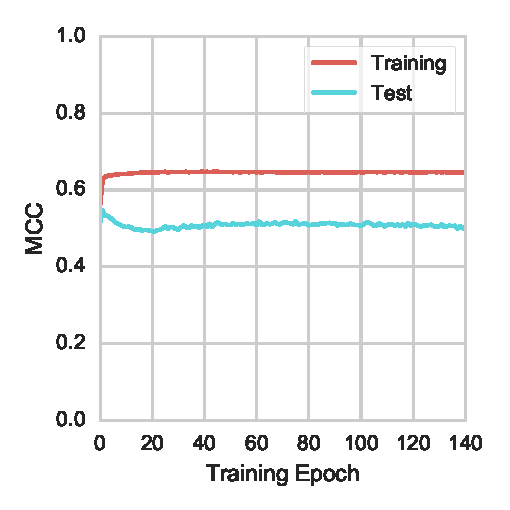
\includegraphics[width=\textwidth]{img/exp-vector-space/doc2vec_training_trained}
      \caption{Training using model vectors}
\label{fig:doc2vec_training_trained}
    \end{subfigure}
    \begin{subfigure}[b]{0.49\textwidth}
      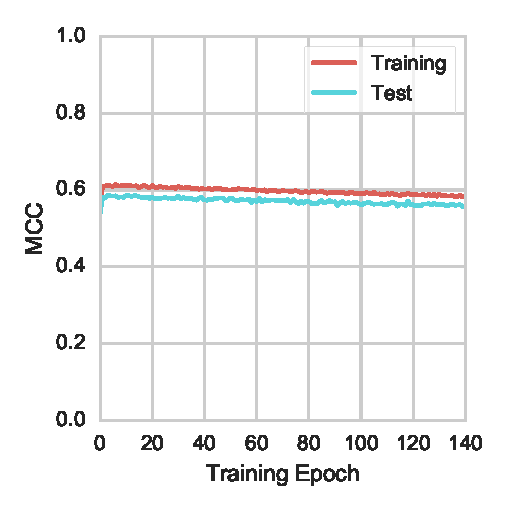
\includegraphics[width=\textwidth]{img/exp-vector-space/doc2vec_training_inferred}
    \caption{Training using inferred vectors}
\label{fig:doc2vec_training_inferred}
    \end{subfigure}
\caption{Comparison of performance when trained the classifier on the trained vectors of the Paragraph Vector model or when inferring new Paragraph Vector vectors for the training data using the model.}
\label{fig:doc2vec_training}
\end{figure}

Lastly the best configurations of hyper-parameters of these approaches were compared in another experiment. Table~\ref{tab:Paragraph Vector Best Configurations Search} lists the tested settings.

\begin{table}[h]
  \begin{center}
  \begin{tabular}{ l | l }
    \toprule
    Vector Size & 300 \\
    Sub-sampling threshold & No \\
    Hierarchical Softmax & \{ No, Yes \} \\
    Negative Sampling Value & \{ 2, 6, 10 \} \\
    Window Size & \{ 8, 10 \} \\
    Model Type & PV-DBOW \\
    Inference Type & Inferred Vectors \\
    \bottomrule
  \end{tabular}
  \caption{Tested Hyper-parameter configurations to find the best Paragraph Vectors model}
  \label{tab:Paragraph Vector Best Configurations Search}
\end{center}
\end{table}

While a \gls{MCC} test score of 0.574 the lowest amongst the candidates the highest score achieved was 0.618. This setting used a window size of 8, a negative sampling value of 10 and hierarchical softmax.

\clearpage

\subsubsection{Evaluation of Classification Methods}
\label{subs:Evaluation of Classification Methods}

\paragraph{Experimental Setup}
\label{par:Experimental Setup}

From the previous experiments on vector space models the best performing setting of each type was chosen.
Specifically those were the following settings:

\begin{itemize}
  \item \textbf{N-Grams}: Unigrams were used with a dimensionality of 300. No stop words filtering and no vector normalization were applied and while using sub-linear TF and IDF.
  \item \textbf{Bag-Of-Means}: As in the experiments above the approach was simply used with an unweighed arithmetic mean of the word vectors in each sentence.
  \item \textbf{Paragraph Vectors}: PV-DBOW word vectors were generated using inference on the training data, a window size of 8, a negative sampling value of 10, hierarchical softmax and no frequent word sub-sampling.
\end{itemize}

Next a diverse set of classification algorithms representative of the algorithm classes described in Section~\ref{sub:Methods For Classification With Vector Space Models} were applied to the data and evaluated.

% The following model characteristics were chosen for each model:
%
% \begin{itemize}
%   \item \textbf{Logistic Regression} A $C$ value of ${0.01, 0.1, 1, 10}$ was evaluated during cross-validation.
%   \item \textbf{Decision Tree}
%   \item \textbf{Naive Bayes} Bernoulli Naive Bayes% Naive Bayes is Bernoulli
%   \item \textbf{SVM}
%   \item \textbf{kNN}
%   \item \textbf{Random Forest}
%   \item \textbf{Neural Network}
%   \item \textbf{Deep Neural Network}
% \end{itemize}

The dataset was then split into 5 folds to perform \gls{Cross-Validation}. For reproducibility, comparability and to save computational resources the vector representations produced by the three vector space models were precomputed for all folds. Naturally the models were trained on the training data in each fold and applied on the test data to ensure unbiased results.

\clearpage

\begin{wraptable}{r}{0.4\textwidth}
\centering
\begin{tabular}{ r l }
  \toprule
  Method & Ratio \\
  \midrule
  Naive Bayes & 0.970 \\
  Logistic Regression & 0.950 \\
  SVM & 0.808 \\
  Neural Network & 0.770 \\
  Deep Neural Network & 0.764 \\
  Random Forest & 0.759 \\
  kNN & 0.726 \\
  Decision Tree & 0.676 \\
  \midrule
  N-Grams & 0.795 \\
  Bag-Of-Means & 0.763 \\
  Paragraph Vectors & 0.679 \\
  \bottomrule
\end{tabular}
\caption{Test to training score ratio for classifiers and vector space models: For classifiers (top) the best performing vector space model was chosen and for vector space models (bottom) scores are averaged over all classifiers.}
\label{tab:Test/Training Ratio}
\end{wraptable}

\begin{table}[h]
  \begin{center}
    \begin{tabular}{ ll cc }
      \toprule
      Classifier & Vector Space & Training Score & Test Score \\
      \midrule
      \multirow{3}{*}{Logistic Regression}
       & N-Grams & 0.770 & 0.697 \\
       & Bag-of-Means & 0.743 & \textbf{0.706} \\
       & Paragraph Vectors & 0.709 & 0.643 \\
      \midrule
      \multirow{3}{*}{Decision Tree}
       & N-Grams & 0.924 & \textbf{0.625} \\
       & Bag-of-Means & 0.938 & 0.455 \\
       & Paragraph Vectors & 0.994 & 0.290 \\
      \midrule
      \multirow{3}{*}{Naive Bayes}
       & N-Grams & 0.668 & \textbf{0.648} \\
       & Bag-of-Means & 0.498 & 0.491 \\
       & Paragraph Vectors & 0.603 & 0.573 \\
      \midrule
      \multirow{3}{*}{SVM}
       & N-Grams & 0.882 & \textbf{0.713} \\
       & Bag-of-Means & --- & --- \\
       & Paragraph Vectors & 0.831 & 0.683 \\
      \midrule
      \multirow{3}{*}{kNN}
       & N-Grams & 0.929 & 0.642 \\
       & Bag-of-Means & 0.944 & \textbf{0.685} \\
       & Paragraph Vectors & 0.993 & 0.579 \\
      \midrule
      \multirow{3}{*}{Random Forest}
       & N-Grams & 0.924 & \textbf{0.701} \\
       & Bag-of-Means & 0.940 & 0.618 \\
       & Paragraph Vectors & 0.985 & 0.509 \\
      \midrule
      \multirow{3}{*}{Neural Network}
       & N-Grams & 0.911 & 0.709 \\
       & Bag-of-Means & 0.930 & \textbf{0.716} \\
       & Paragraph Vectors & 0.975 & 0.665 \\
      \midrule
      \multirow{3}{*}{Deep Neural Network}
       & N-Grams & 0.913 & 0.708 \\
       & Bag-of-Means & 0.936 & \textbf{0.715} \\
       & Paragraph Vectors & 0.989 & 0.679 \\
      % \midrule
      % \multirow{3}{*}{Convolutional \gls{ANN}}
      % & \multirow{3}{*}{---}
      % & N-Grams & --- & --- \\
      % & & Bag-of-Means & --- & --- \\
      % & & Paragraph Vectors & --- & --- \\
      \bottomrule
    \end{tabular}
  \caption{Test and Training performance in terms of \gls{MCC} for the whole set of classifiers. Each classifier was applied to data transformed using the best configuration for each of the three vector space model classes}
\label{tab:Classifier Results}
\end{center}
\end{table}

\paragraph{Generalization Performance}
\label{par:Generalization Performance}

We will first take a look at the results in terms of their capability to generalized the learned structure from the training data. In indicator for this ability is the ratio between performance on test and training data. Table~\ref{tab:Test/Training Ratio} shows a comparison in terms of this ration between both the classification algorithms as well as the vector space models when averaged over the performance with all algorithms. The results are sorted in order of their score which was measured in terms of \gls{MCC} as mentioned previously.

Regarding the classifiers we can observe that Naive Bayes and Logistic Regression achieve a very high ratio signaling successful generalization.
% Looking at Table~\ref{tab:Paragraph Vector Parameter Hyper-Parameter Results} we can see that the algorithms also both perform considerably well
For the Neural Networks models tested it is apparent that the deep architecture overfits more than the network with a single hidden layer, i.e. it achieves higher training but lower test scores. When comparing the Deep Neural Network to Random Forests using Paragraph Vectors though we can see that while both methods achieve similarly high scores on the training data, Random Forests perform significantly worse on the test data --- Random Forests achieve scores of 0.985 (training) and 0.509 (test) as opposed to the scores of 0.989 (training) and 0.679 (test) for the Deep Neural Network. In such a setting we can expect these methods to increase the level of overfitting when the dataset size is increased.


\paragraph{Performance of Vector Space Models with Different Classifiers}
\label{par:Performance of Vector Space Models with Different Classifiers}

A set of methods achieve remarkable performance with simple N-Grams. Among them the SVM ranks highest with a \gls{MCC} test score of 0.713. Interestingly though in many cases the training score using Paragraph Vectors is highest, including both Tree-based methods, the Neural Network approaches and \gls{kNN}. This means that in principle they offer a better representation of the data to the algorithm, making it possible overfit on the rather small dataset. This is also shown in Table~\ref{par:Generalization Performance} where Paragraph Vectors show a 10\% decreased generalization performance, meaning that on average the classifiers tend to overfit on this representation.
Another important result is that the Bag-of-Means model performs best overall and this is consistent half of the classifiers. The highest test score of 0.716 was achieved by a Neural Network using this model.

\paragraph{Comparison of Classifiers}
\label{par:Comparison of Classifiers}




naive bayes does strange things (BOM vs Ngram)

N-grams
- In many cases still best performance
-



Vector Spaces compared:


First of all we note that in none of the setups paragraph vectors performed best. Vectors produced with the  Bag-Of-Means approach however did outperform the N-gram model in in combination with some of the classifiers, namely Logistic Regression, \gls{kNN} and the Neural Network models of which the simple Neural Network achieved a test score of 0.716 using this technique, the highest test score of all classifiers.

% Regarding vector spaces
- Ngrams are best in most settings
- Bag of means performs pretty well considering that it was reported not to
- paragraph vectors often on par but don't outperform (probably need more data)
- PV seem to make models overfit in many cases (knn, NN, DNN)

- SVM is good
- DNN overfits (probably)
-


\paragraph{Overall test performance}
\label{par:Overall test performance}

\begin{table}[h]
  \begin{center}
    \begin{tabular}{ l c c c }
      \toprule
      Algorithm & N-Grams & Bag-Of-Means & Paragraph Vectors \\
      \midrule
      Data Transformation & 0.68s & 1.49m & 5.31h \\
      \midrule
      Logistic Regression & 32.08s & 2.15m & 6.26m \\
      Decision Tree & 30.05s & 4.47m & 4.85m \\
      Naive Bayes & 1.33s & 12.29s & 12.07s \\
      SVM & 15.53m & 1.30h & 1.60h \\
      kNN & 4.24s & 1.16h & 1.23h \\
      Random Forest & 14.82m & 4.24h & 5.65h \\
      \midrule
      Neural Network & 21.32m & 21.26m & 21.04m \\
      Deep Neural Network & 32.84m & 32.65m & 32.22m \\
      \bottomrule
    \end{tabular}
  \caption{Computation time for the experiments. The top row shows the time for generating the feature space models and the rest of the results show the runtime for the different classifiers. The neural network models are separated because they were trained on an Amazon AWS \emph{g2.2xlarge} \gls{GPU} instance while the other models were trained on \emph{c4.large} instance using a multi-core CPU. The runtime of all classifiers includedes 5-fold \gls{Cross-Validation} and grid-search over hyper-parameters for most models. Thus the results are only representative to a certain extent as some models had a smaller hyper-parameter space to be evaluated.}
\label{tab:Computation}
\end{center}
\end{table}

\subsection{Classification With Sequential Models}
\label{sub:Classification With Sequential Models}


\begin{table}[h]
  \begin{center}
    \begin{tabular}{ l c c c }
      \toprule
      Model & Training Loss & Test Loss & Test Score \\
      \midrule
      Simple LSTM & 0.733 & 0.767 & 0.689 \\
      Stacked LSTM & 0.674 & 0.791 & \textbf{0.707} \\
      Multi-task LSTM & --- & --- & 0.258 \\
      \bottomrule
    \end{tabular}
  \caption{Test and training scores for the LSTM recurrent neural network models. Due to limited computational resources the \gls{MCC} score was only evaluated at test time while measuring the categorical cross-entropy loss during training and also at test time.}
\label{tab:LSTM Results}
\end{center}
\end{table}

\subsubsection{Character-based LSTM *}

\subsubsection{Stacked Character-based LSTM *}

\subsubsection{Character-based Multi-task LSTM *}
